\part{Agrégats, mémoire et fichiers }
\label{agrégats,-mémoire-et-fichiers }

\chapter{Les pointeurs}
\label{les-pointeurs}

Dans ce chapitre, nous allons aborder une notion centrale du langage C~: les pointeurs.

Les pointeurs constituent ce qui est appellé une \textbf{fonctionnalité
bas niveau}, c'est-à-dire un mécanisme qui nécessite de connaître
quelques détails sur le fonctionnement d'un ordinateur pour être compris
et utilisé correctement. Dans le cas des pointeurs, il s'agira surtout
de disposer de quelques informations sur la mémoire vive.

\section{Présentation}
\label{presentation}

Avant de vous présenter le concept de
pointeur, un petit rappel concernant la mémoire s'impose (n'hésitez pas
à relire le chapitre sur les variables si celui-ci s'avère insuffisant).

Souvenez-vous : toute donnée manipulée par l'ordinateur est stockée dans
sa \textbf{mémoire}, plus précisément dans une de ses différentes
mémoires (registre(s), mémoire vive, disque(s) dur(s), etc.). Cependant,
pour utiliser une donnée, nous avons besoin de savoir où elle se situe,
nous avons besoin d'une \textbf{référence} vers cette donnée. Dans la
plupart des cas, cette référence est en fait une \textbf{adresse
mémoire} qui indique la position de la donnée dans la mémoire vive.

\subsection{Les pointeurs}
\label{les-pointeurs-1}

Si l'utilisation des références peut être implicites (c'est par exemple
le cas lorsque vous manipulez des variables), il est des cas où elle
doit être explicite. C'est à cela que servent les \textbf{pointeurs} :
ce sont des variables dont le contenu est une adresse mémoire (une
référence, donc).

\begin{figure}[htbp]
\centering
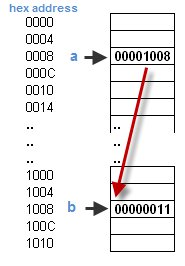
\includegraphics[scale=0.7]{images/pointeur.jpg}
\caption{Exemple, avec une variable a qui est un pointeur sur une
variable b}
\end{figure}

\subsection{Utilité des pointeurs}
\label{utilite-des-pointeurs}

Techniquement, il y a trois utilisations majeures des pointeurs en C :

\begin{itemize}
\item
  le passage de références à des fonctions ;
\item
  la manipulation de données complexes ;
\item
  l'allocation dynamique de mémoire.
\end{itemize}

\subsubsection{Passage de références à des fonctions}
\label{passage-de-references-a-des-fonctions}

Rappelez-vous du chapitre sur les fonctions : lorsque vous fournissez un
argument lors d'un appel, la valeur de celui-ci est affectée au
paramètre correspondant, paramètre qui est une variable propre à la
fonction appelée. Toutefois, il est parfois souhaitable de modifier une
variable de la fonction \emph{appelante}. Dès lors, plutôt que de passer
la valeur de la variable en argument, c'est une référence vers celle-ci
qui sera envoyée à la fonction.

\subsubsection{Manipulation de données complexes}
\label{manipulation-de-donnees-complexes}

Jusqu'à présent, nous avons manipulé des données simples : \mybox{int},
\mybox{double}, \mybox{char}, etc. Cependant, le C nous permet
également d'utiliser des données plus complexes qui sont en fait des
\textbf{agrégats} (un regroupement si vous préférez) de données simples.
Or, il n'est possible de manipuler ces agrégats qu'en les parcourant
données simples par données simples, ce qui requiert de disposer d'une
référence vers les données qui le composent.

\begin{infobox}
Nous verrons les agrégats plus en détails lorsque nous aborderons les
structures et les tableaux.
\end{infobox}


\subsection{L'allocation dynamique de mémoire}
\label{lallocation-dynamique-de-memoire}

Il n'est pas toujours possible de savoir quelle quantité de mémoire sera
utilisée par un programme. En effet, si vous prenez le cas d'un logiciel
de dessin, ce dernier ne peut pas prévoir quelle sera la taille des
images qu'il va devoir manipuler. Pour palier à ce problème, les
programmes recours au mécanisme de l'\textbf{allocation dynamique de
mémoire} : ils demandent de la mémoire au système d'exploitation lors de
leur exécution. Pour que cela fonctionne, le seul moyen est que le
système d'exploitation fournisse au programme une référence vers la zone
allouée.

\section{Déclaration et initialisation}
\label{declaration-et-initialisation-1}

La syntaxe pour déclarer un pointeur est la suivante.

\begin{C}
type *nom_du_pointeur;
\end{C}

Par exemple, si nous souhaitons créer un pointeur sur \mybox{int}
(c'est-à-dire un pointeur pouvant stocker l'adresse d'un objet de type
\mybox{int}) et que nous voulons le nommer « ptr », nous devons écrire
ceci.

\begin{C}
int *ptr;
\end{C}

L'astérisque peut être entourée d'espaces et placée n'importe où entre
le type et l'identificateur. Ainsi, les trois définitions suivantes sont
identiques.

\begin{C}
int *ptr;
int * ptr;
int* ptr;
\end{C}

\begin{attentionbox}
Notez bien qu'un pointeur est toujours typé. Autrement dit, vous aurez
toujours un pointeur sur (ou vers) un objet d'un certain type (\mybox{int},
\mybox{double}, \mybox{char}, etc.).
\end{attentionbox}

\subsection{Initialisation}
\label{initialisation-2}

Un pointeur, comme une variable, ne possède pas de valeur par défaut, il
est donc important de l'initialiser pour éviter d'éventuels problèmes.
Pour ce faire, il est nécessaire de recourir à l'\textbf{opérateur
d'adressage} (ou de référencement) : \mybox{\&} qui permet d'obtenir
l'adresse d'un objet. Ce dernier se place derrière l'objet dont
l'adresse souhaite être obtenue. Par exemple comme ceci.

\begin{C}
int a = 10;
int *p;

p = &a;
\end{C}

Ou, plus directement, comme cela.

\begin{C}
int a = 10;
int *p = &a;
\end{C}

\begin{erreurbox}
Faites bien attention à ne pas mélanger différents types de pointeurs !
Un pointeur sur \mybox{int} n'est pas le même qu'un pointeur sur \mybox{long}
ou qu'un pointeur sur \mybox{double}. De même, n'affectez l'adresse d'un
objet qu'à un pointeur du même type.
\begin{C}
 int a;
double b;
int *p = &b; /* faux */
int *q = &a; /* correct */
double *r = p; /* faux */
\end{C}
\end{erreurbox}

\subsection{Pointeur nul}
\label{pointeur-nul}

Vous souvenez-vous du chapitre sur la gestion d'erreur ? Dans ce
dernier, nous vous avons dit que, le plus souvent, les fonctions
retournaient une valeur particulière en cas d'erreur. \emph{Quid} de
celles qui retournent un pointeur ? Existe-t-il une valeur spéciale qui
puisse représenter une erreur ou bien sommes-nous condamner à utiliser
une variable globale comme \mybox{errno} ?

Heureusement pour nous, il existe un cas particulier : les pointeurs
nuls. Un pointeur nul est tout simplement un pointeur contenant une
adresse invalide. Cette adresse invalide dépend de votre système
d'exploitation, mais elle est la même pour tous les pointeurs nuls.
Ainsi, deux pointeurs nuls ont une valeur égale.

Pour obtenir cette adresse invalide, il vous suffit de convertir
explicitement zéro vers le type de pointeur voulu. Ainsi, le pointeur
suivant est un pointeur nul.

\begin{C}
int *p = (int *)0;
\end{C}

\begin{infobox}
Rappelez-vous qu'il y a conversion implicite vers le type de destination
dans le cas d'une affectation. La conversion est donc superflue dans ce cas-ci. 
\end{infobox}


\subsubsection{La constante NULL}
\label{la-constante-null}

Afin de clarifier un peu les codes sources, il existe une constante
définie dans l'en-tête \mybox{\textless{}stddef.h\textgreater{}} :
\mybox{NULL}. Celle-ci peut être utilisée partout où un pointeur nul
est attendu \emph{sauf comme argument de la fonction \mybox{printf()}}
(nous verrons pourquoi plus tard dans ce cours).

\begin{C}
int *p = NULL; /* Un pointeur nul. */
\end{C}

\section{Utilisation }
\label{utilisation-2}

\subsection{Indirection (ou déréférencement)}
\label{indirection-(ou déréférencement)}

Maintenant que nous savons récupérer l'adresse d'un objet et l'affecter
à un pointeur, voyons le plus intéressant : accéder à cet objet ou le
modifier via le pointeur. Pour y parvenir, nous avons besoin de
l'\textbf{opérateur d'indirection} (ou de déréférencement) : \mybox{*}.

\begin{questionbox}
 Le symbole \mybox{*} n'est pas celui de la multiplication ? 
\end{questionbox}

Si, c'est aussi le symbole de la multiplication. Toutefois, à l'inverse
de l'opérateur de multiplication, l'opérateur d'indirection ne prends
qu'un seul opérande (il n'y a donc pas de risque de confusion).

L'opérateur d'indirection attends un pointeur comme opérande et se place
juste derrière celui-ci. Une fois appliqué, ce dernier nous donne accès
à la valeur de l'objet référencé par le pointeur, aussi bien pour la
lire que pour la modifier.

Dans l'exemple ci-dessous, nous accédons à la valeur de la variable
\mybox{a} via le pointeur \mybox{p}.

\begin{C}
int a = 10;
int *p = &a;

printf("a = %d\n", *p);
\end{C}

\begin{C}
a = 10
\end{C}

À présent, modifions la variable \mybox{a} à l'aide du pointeur
\mybox{p}.

\begin{C}
int a = 10;
int *p = &a;

*p = 20;
printf("a = %d\n", *p);
\end{C}

\begin{C}
a = 20
\end{C}

\begin{infobox}
Comme pour n'importe quelle variable,
il est possible de déclarer un pointeur comme constant. Cependant,
puisqu'un pointeur référence un objet, il peut également être déclaré
comme un pointeur vers un objet constant. Pour ce faire, la position du
mot-clé \mybox{const} est importante. Si le
mot-clé est devant l'identificateur et derrière le symbole \mybox{*},
alors il s'agit d'un pointeur constant.
\begin{C}
int * const ptr; /* Un pointeur constant sur int. */
\end{C}

Si le mot-clé est devant le symbole \mybox{*} et derrière le type référencé, alors il s'agit d'un pointeur vers un objet
constant. 

\begin{C}
int const *ptr; /* Pointeur sur int constant. */
\end{C}

Enfin, ces deux notations peuvent être combinées
pour créer un pointeur constant vers un objet constant. 

\begin{C}
int const * const ptr; /* Pointeur constant sur int constant. */
\end{C}
\end{infobox}

\subsection{Passage comme argument}
\label{passage-comme-argument}

Voici un exemple de passage de pointeurs en arguments d'une fonction.

\begin{C}
#include <stdio.h>

void test(int *pa, int *pb)
{
    *pa = 10;
    *pb = 20;
}


int main(void)
{
    int a;
    int b;
    int *pa = &a;
    int *pb = &b;

    test(&a, &b);
    test(pa, pb);
    printf("a = %d, b = %d\n", a, b);
    printf("a = %d, b = %d\n", *pa, *pb);
    return 0;
}
\end{C}

\begin{C}
a = 10, b = 20
a = 10, b = 20
\end{C}

Remarquez que les appels \mybox{test(\&a,\ \&b)} et
\mybox{test(pa,\ pb)} réalisent la même opération.

\section{Retour de fonction}\label{retour-de-fonction}

Pour terminer, sachez qu'une fonction peut également retourner un
pointeur. Cependant, faites attention : \emph{l'objet référencé par le
pointeur doit toujours exister au moment de son utilisation} ! L'exemple
ci-dessous est donc incorrect étant donnée que la variable \mybox{n}
est de classe de stockage automatique et qu'elle n'existe donc plus
après l'appel à la fonction \mybox{ptr()}.

\begin{C}
#include <stdio.h>


int *ptr(void)
{
    int n;

    return &n;
}


int main(void)
{
    int *p = ptr();

    *p = 10;
    printf("%d\n", *p);
    return 0;
}
\end{C}

L'exemple devient correct si \mybox{n} est de classe de stockage
statique.

\section{Pointeur de pointeur}\label{pointeur-de-pointeur}

Au même titre que n'importe quel autre objet, un pointeur a lui aussi
une adresse. Dès lors, il est possible de créer un objet pointant sur ce
pointeur : un pointeur de pointeur.

\begin{C}
int a = 10;
int *pa = &a;
int **pp = &pa;
\end{C}

Celui-ci s'utilise de la même manière qu'un pointeur si ce n'est qu'il
est possible d'opérer deux indirections : une pour atteindre le pointeur
référencé et une seconde pour atteindre la variable sur laquelle pointe
le premier pointeur.

\begin{C}
#include <stdio.h>


int main(void)
{
    int a = 10;
    int *pa = &a;
    int **pp = &pa;

    printf("a = %d\n", **pp);
    return 0;
}
\end{C}

\begin{infobox}
Ceci peut continuer à l'infini pour concevoir 
des pointeurs de pointeur de pointeur de pointeur de\ldots{}
Bref, vous avez compris le principe.
\end{infobox}

\section{Pointeurs génériques et affichage}
\label{pointeurs-generiques-et-affichage}

\# Le type \mybox{void}

Vous avez déjà recontré le mot-clé \mybox{void} lorsque nous avons
parlé des fonctions, ce dernier permet d'indiquer qu'une fonction
n'utilise aucun paramètre et/ou ne retourne aucune valeur. Toutefois,
nous n'avons pas tout dit à son sujet : \mybox{void} est en fait un
type, au même titre que \mybox{int} ou \mybox{double}. o\_O

\begin{questionbox}
Et il représente quoi ce type, alors ?
\end{questionbox}


\emph{Hum}\ldots{} rien (d'où son nom). :-°\\
En fait, il s'agit d'un type dit « \textbf{incomplet} », c'est à dire
que la taille de ce dernier n'est pas calculable et qu'il n'est pas
utilisable dans des expressions. Quel est l'intérêt de la chose me
direz-vous ? Permettre de créer des pointeurs « \textbf{génériques} »
(ou « universels »).

En effet, nous venons de vous dire qu'un pointeur devait toujours être
typé. Cependant, cela peut devenir gênant si vous souhaitez créer une
fonction qui doit pouvoir travailler avec n'importe quel type de
pointeur (nous verrons un exemple très bientôt). C'est ici que le type
\mybox{void} intervient : un pointeur sur \mybox{void} est considéré
comme un pointeur générique, ce qui signifie qu'il peut référencer
n'importe quel type d'objet.

En conséquence, il est possible d'affecter n'importe quelle adresse
d'objet à un pointeur sur \mybox{void} et d'affecter un pointeur sur
\mybox{void} à n'importe quel autre pointeur (et inversément).

\begin{C}
int a;
double b;
void *p;
double *r;

p = &a; /* correct */
p = &b; /* correct */
r = p; /* correct */
\end{C}

\section{Afficher une adresse}\label{afficher-une-adresse}

Il est possible d'afficher une adresse à l'aide de l'indicateur de
conversion \mybox{p} de la fonction \mybox{printf()}. Ce dernier
attends en argument un pointeur sur \mybox{void}. Vous voyez ici
l'intérêt d'un pointeur générique : un seul indicateur suffit pour
afficher tous les types de pointeurs.

Notez que l'affichage s'effectue le plus souvent en hexadécimal.

\begin{C}
int a;
int *p = &a;

printf("%p == %p\n", (void *)&a, (void *)p);
\end{C}

Tant que nous y sommes, profitons en pour voir quelle est l'adresse
invalide de notre système.

\begin{C}
printf("%p\n", (void *)0);
\end{C}

\begin{secretbox}
Oui, le plus souvent, il s'agit de zéro. 
\end{secretbox}


\section{Exercice}
\label{exercice-12}


Pour le moment, tout ceci doit sans doute vous paraître quelques peu 
abstrait et sans doute inutile. Toutefois, rassurez-vous, cela vous semblera
plus clair après les chapitres suivants.

En attendant, nous vous proposons un petit exercice mettant en pratique
les pointeurs : programmez une fonction nommée « swap », dont le rôle
est d'échanger la valeur de deux variables de type \mybox{int}.
Autrement dit, la valeur de la variable « a » doit devenir celle de « b
» et la valeur de « b », celle de « a ».

\section{Correction}
\label{correction-14}

\begin{C}
 #include <stdio.h>

void swap(int *, int *);


void swap(int *pa, int *pb)
{
    int tmp;

    tmp = *pa;
    *pa = *pb;
    *pb = tmp;
}


int main(void)
{
    int a = 10;
    int b = 20;

    swap(&a, &b);
    printf("a = %d, b = %d\n", a, b);
    return 0;
}
\end{C}

\hrulefill

Nous en avons fini avec les pointeurs, du moins, pour le moment.

En effet, les pointeurs sont omniprésents en langage C et nous n'avons
pas fini d'en entendre parler. Mais pour l'heure, nous allons découvrir
une des fameuses données complexes dont nous avons parlé en début de
chapitre : les \textbf{structures}.